\documentclass[12pt]{report}
\usepackage{amsmath}
\usepackage{graphicx}
\title{Project 1:Exploring Weather Trends}
\author{Jared Thacker}

\begin{document}
\maketitle

\chapter{Report}
\section{ Outline}
In this project PostgreSQL was used to obtain both the global and local Atlanta temperature data from a database kept by Udacity.  The SQL statements to extract the Atlanta temperature data is:\\

\noindent SELECT * \\
FROM city\textunderscore data \\
WHERE country = 'United States' AND city = 'Atlanta'\\
LIMIT 100 \\

\noindent And the SQL statements to extract the global temperature data is: \\

\noindent SELECT * \\
FROM global\textunderscore data \\

\noindent Python, with the pandas and matplotlib libraries, was then used to load and visualize the data. The rolling mean method from pandas was used to calculate the moving average with a window of 5. This means that the previous 5 data points (including the current data point) were used to calculate the average at the current point in time.  A window of $n = 20$ was initially chosen but tended to smooth out the curve too much, so a window of $n = 5$ was settled upon and maintained the noise in the graph, but also captured the trend in the data well.
\begin{figure}
	\center{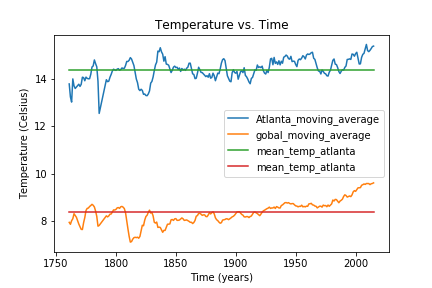
\includegraphics[width=\textwidth]
        {globalAndAtlanta.png}}
        \caption{\label{fig:atlantaDataAndTrend} The Atlanta temperature data and moving average to show the trend in the data.}
\end{figure}

\begin{figure}
	\center{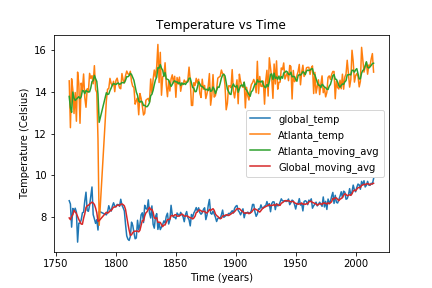
\includegraphics[width = \textwidth]
	{globalAndAtlantaRawData.png}}
	\caption{\label{fig:globalDataAndTrend} The global temperature data and moving average to show the trend in the data.}
\end{figure}

\section{Observations}
The moving averages definitely show that the average global temperature increases as time has passed, however, it is rather unclear with the Atlanta data. In addition, the Atlanta moving average tends to dip and peak in the same place as does the global moving average; this is most easily seen in at approximately year 1825 by comparing the moving averages between the two plots. Third, the temperature in Atlanta is definitely warmer than the global average temperature; the Atlanta temperature is only lower than the global average at one point in time. Lastly, while both temperature trends increase as time passes, the increase in global temperature is more dramatic than Atlanta's as can be seen when comparing the moving averages.\\

\noindent In figure (\ref{fig:atlantaDataAndTrend}), the moving average and mean temperatures for the globe and Atlanta are plotted in the same figure and in figure (\ref{fig:globalDataAndTrend}) the raw time-series and moving averages are plotted both globally and for Atlanta. In the paragraphs that follow, visual inspection as well as the Dickey-Fuller test is used to come to conclusions about the data.\\

\noindent If we visually inspect the raw data (orange curve) for Atlanta in figure (\ref{fig:globalDataAndTrend}) there does not seem to be an upward trend (values get steadily larger) or a downward trend (values get steadily smaller). In addition, there does not seem to be significantly large differences in each value in the time-series with the exception in the late 1700s which implies a constant variance in time in this time-series. Therefore, upon visual inspection, it looks like the Atlanta data is stationary and has no trend. In figure (\ref{fig:atlantaDickeyFullerTest}), the results of the Dickey-Fuller test performed on the Atlanta data are given. Since the test statistic is smaller any of the critical values, we can conclude that the data Atlanta is stationary. This means that, at least with the data collected so far, there is no trend in the Atlanta data that shows that temperature is increasing or varying signifcantly. \\

\begin{figure}
	\center{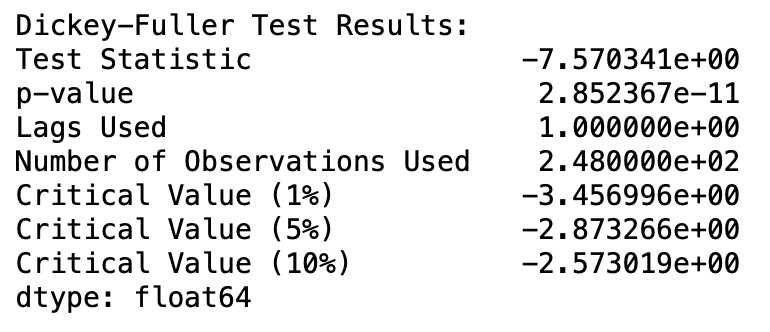
\includegraphics[width = \textwidth]
	{atlantaDickeyFullerTest.png}}
	\caption{\label{fig:atlantaDickeyFullerTest} The results of the Dickey-Fuller test for the Atlanta data.}
\end{figure}

\noindent If we visually inspect the raw (blue curve) for the global data in figure (\ref{fig:globalDataAndTrend}) there is definitely an upward trend (values get larger). This can be seen more clearly in figure (\ref{fig:atlantaDataAndTrend}) where the values past around 1925 seem to \textit{stay} above the mean (the red horizontal line).  In addition, the variance seems to decrease as time goes on since the difference between the values seems to decrease as time goes on. Therefore, upon visual inspection, the global time-series data is non-stationary and exhibits trends, the most important of which that the average global temperature is increasing as time passes (global warming). We can confirm this by referring to the Dickey-Fuller test in figure (\ref{fig:globalDickeyFullerTest}) . The test statistic is not smaller than any of the critical values which means that we cannot reject that the time-series is non-stationary. Therefore, by visual comparison and by the Dickey-Fuller test, the global time-series has an upwards (increasing) trend and is non-stationary. Therefore, we can conclude that the average temperature of the earth is increasing. 

\begin{figure}
	\center{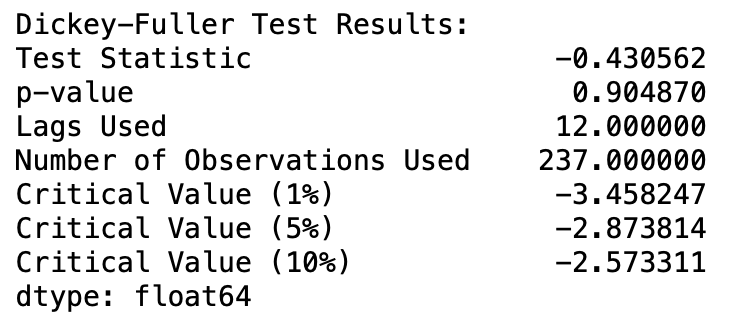
\includegraphics[width = \textwidth]
	{globalDickeyFullerTest.png}}
	\caption{\label{fig:globalDickeyFullerTest} The results of the Dickey-Fuller test for the global data.}
\end{figure}

\end{document}

